\section{Assignment 4}

\subsection{Compute cubic splines based on the accelerations with assigned initial and final velocities.}

The interpolation based on accelerations is centred around the solution of the system of linear equations:

\begin{align*}
A\ddot q &= c\\
\begin{bmatrix}
2T_0 & T_0 & 0\\
T_0 & 2(T_0+T_1) & T_0 & 0\\
& \ddots & \ddots & \ddots \\
& & T_k & 2(T_k+T_{k+1}) & T_{k+1}\\
& & & \ddots & \ddots & \ddots\\
& & & & T_{n-2} & 2(T_{n-2}+T_{n-1})& T_{n-1}\\
& & & & & T_{n-1} & 2T_{n-1}\\
\end{bmatrix}\begin{bmatrix}
\ddot q_0\\\vdots\\\ddot q_k\\\vdots\\\ddot q_n
\end{bmatrix}&=\begin{bmatrix}
6\left(\frac{q_1-q_0}{T_0}-\dot q_0\right)\\
\vdots\\
6\left(\frac{q_k-q_{k-1}}{T_{k-1}}-\frac{q_{k-1}-q_{k-2}}{T_{k-2}}\right)\\
\vdots\\
6\left(\dot q_n-\frac{q_{n}-q_{n-1}}{T_{n-1}}\right)
\end{bmatrix}
\end{align*}

Thanks to the tridiagonal form of matrix $A$, the system can be solved with Thomas' algorithm.

\begin{figure}[h]
\centering
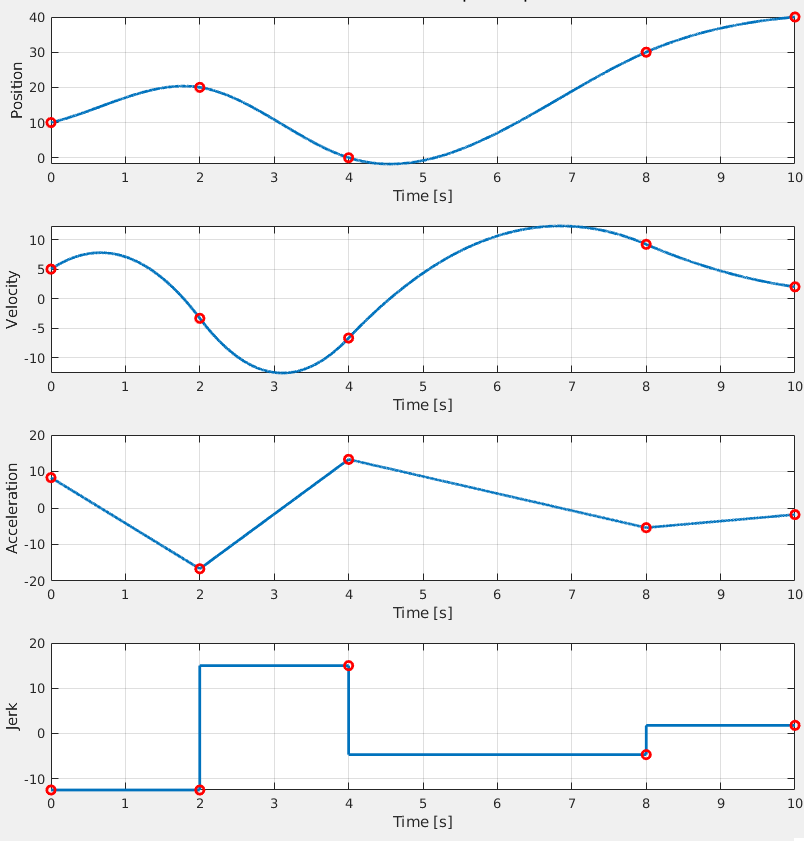
\includegraphics[keepaspectratio,width=0.8\textwidth]{smooth_1}
\caption{Trajectory based on accelerations through $q_k=\begin{bmatrix}
10 & 20 & 0 & 30 & 40
\end{bmatrix}$ at times $t_k=\begin{bmatrix}
0 & 2 & 4 & 8 & 10
\end{bmatrix}$ with $\dot q_i=5$ and $\dot q_f=2$.}
\end{figure}

\newpage

\subsection{Compute the smoothing cubic splines.}

The smoothing cubic splines express a trade-off between the fitting of the given points and the minimization of the curvature and acceleration of the trajectory, through a parameter $\mu$. The closeness of the approximation is expressed by a weight vector $w$, which weighs every point in the trajectory. The closer $w_k$ is to zero, the closer the resulting trajectory is to the interpolation of the point.

\begin{figure}[h]
\centering
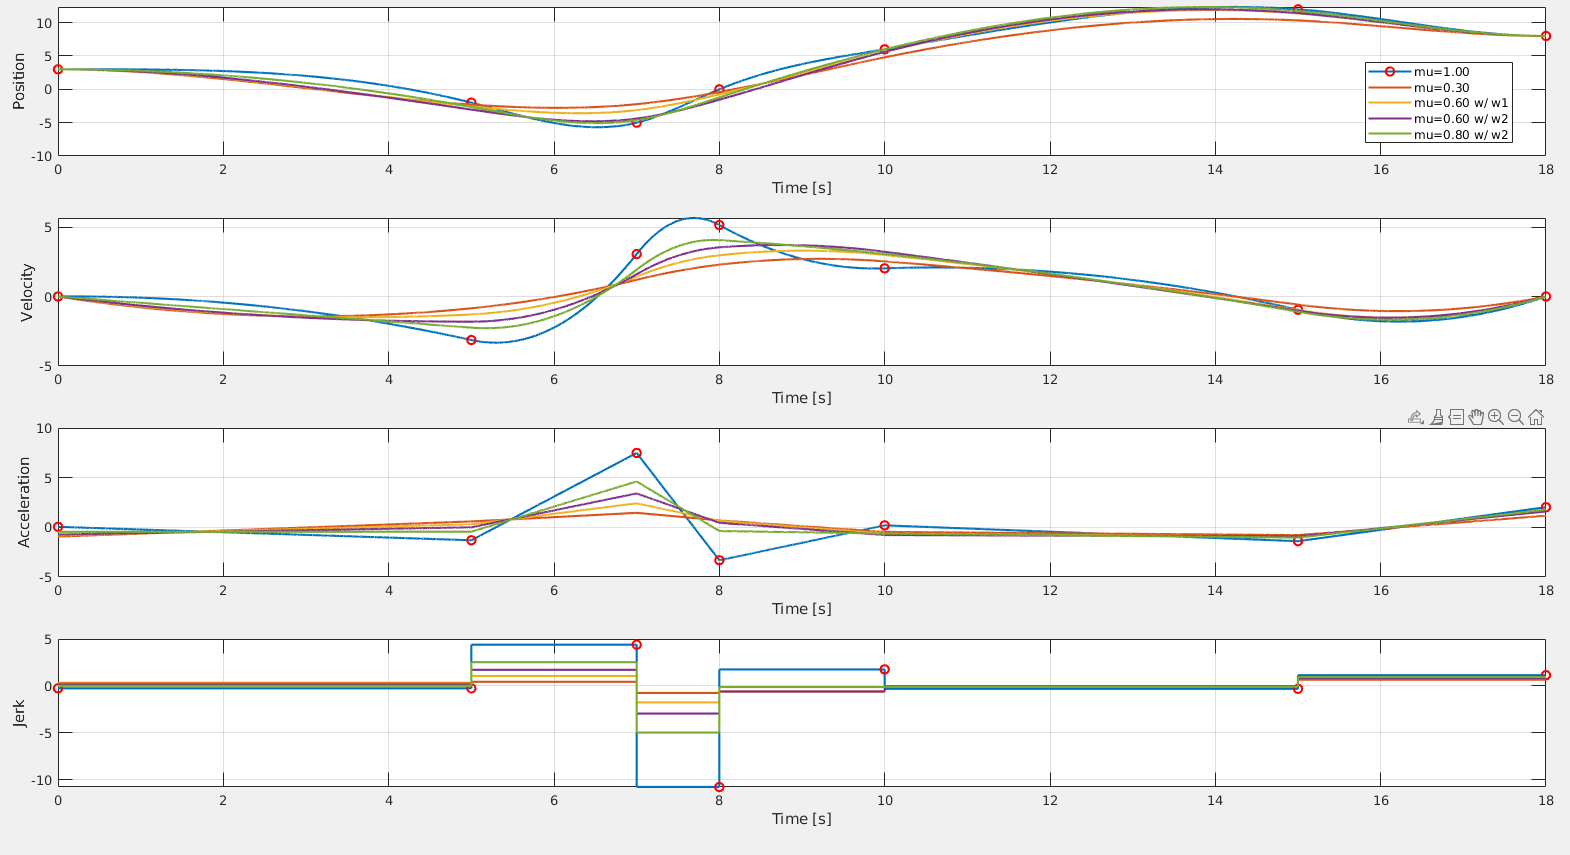
\includegraphics[height=0.6\textheight ,width=\textwidth]{smooth_2}
\caption{Comparison of smoothing cubic splines. $w1=\begin{bmatrix}
\infty &1 &1 &1 &1 &1 &\infty
\end{bmatrix}$,$w2=\begin{bmatrix}
\infty &1 &5 &1 &1 &1 &\infty
\end{bmatrix}$. Note that the actual used value is $1/w_k$.}
\end{figure}
